\subsection{The Typical CNN Architecture}\label{sec:typical-cnn-architecture}

The previous section introduced the basic computational idea: apply local filters to an image. Now we will show how these operations are organized into a complete CNN.

\highspace
The central change is that the network no longer processes a single filtered image. Instead, it \textbf{repeatedly transforms the input} into a \textbf{sequence of multi-channel volumes} until it eventually obtains a vector suitable for a traditional classifier.

\highspace
First of all, the \hl{\textbf{input} of a CNN is an entire image.} This distinguishes CNNs from the hand-crafted pipeline discussed earlier:
\begin{equation*}
    \text{Image} \to \text{Manually Extracted Vector of Features} \to \text{Classifier}
\end{equation*}
Now, the CNN takes the image as input and automatically learns the features:
\begin{equation*}
    \text{Image} \to \text{CNN}
\end{equation*}
The \textbf{network} itself is \textbf{responsible for transforming the image into useful features}.

\highspace
For a color image, the input is naturally represented as a \textbf{3D vector}:
\begin{equation*}
    \mathbf{x} \in \mathbb{R}^{H \times W \times C}
\end{equation*}
Where $H$ is the image height, $W$ is the image width, and $C$ is the number of channels (3 for RGB images, 1 for grayscale images).

\highspace
Usually, the input image of a CNN is called \important{input volume}. An ordinary image is often drawn as a two-dimensional rectangle. However, a color image contains three values at every spatial position:
\begin{equation*}
    x(r, c, 1), \quad x(r, c, 2), \quad x(r, c, 3)
\end{equation*}
These correspond to the red, green, and blue channels of the image. Therefore, the image has three dimensions:
\begin{equation*}
    \text{Height} \times \text{Width} \times \text{Channels}
\end{equation*}
It can be visualized as a stack of $C$ two-dimensional maps:
\begin{equation*}
    \mathbf{x} = \begin{bmatrix}
        \text{channel }1 \\
        \text{channel }2 \\
        \vdots \\
        \text{channel }C
    \end{bmatrix}
\end{equation*}
This stack of channels is called a \important{volume}. The depth here means number of channels, not physical depth in the sense of 3D space.

\begin{examplebox}[: Input Volume]
    Suppose the image is only $2 \times 2$ pixels. Its three channels might be:
    \begin{equation*}
        R = \begin{bmatrix}
            10 & 20 \\
            30 & 40
        \end{bmatrix},
        \quad
        G = \begin{bmatrix}
            50 & 60 \\
            70 & 80
        \end{bmatrix},
        \quad
        B = \begin{bmatrix}
            90 & 100 \\
            110 & 120
        \end{bmatrix}
    \end{equation*}
    Each channel is still a $2 \times 2$ matrix. Stacking them produces one three-dimensional array:
    \begin{equation*}
        I \in \mathbb{R}^{2 \times 2 \times 3}
    \end{equation*}
    Defined by:
    \begin{equation*}
        I(:,:,1) = R, \quad I(:,:,2) = G, \quad I(:,:,3) = B
    \end{equation*}
    Conceptually, the input volume can be visualized as a stack of three $2 \times 2$ matrices, one for each channel:
    \begin{equation*}
        I = \begin{bmatrix}
            R \\
            G \\
            B
        \end{bmatrix}
    \end{equation*}
    The brackets do \textbf{not} mean ordinary vertical matrix concatenation. They mean that the matrices occupy different slices along a new dimension. Thus, at spatial position $(1, 2)$, the corresponding values are:
    \begin{equation*}
        R(1, 2) = 20, \quad G(1, 2) = 60, \quad B(1, 2) = 100
    \end{equation*}
    Therefore:
    \begin{equation*}
        I(1, 2, :) = \begin{bmatrix}
            20 \\
            60 \\
            100
        \end{bmatrix}
    \end{equation*}
    So every spatial position contains an RGB triplet:
    \begin{equation*}
        I(r, c, :) = \begin{bmatrix}
            R(r, c) \\
            G(r, c) \\
            B(r, c)
        \end{bmatrix}
    \end{equation*}
    The structure is therefore:
    \begin{center}
        \begin{tabular}{@{} c c @{}}
            \toprule
            \textbf{Spatial Position} & \textbf{Values along depth} \\
            \midrule
            $(1, 1)$ & $[10,\; 50,\; 90]$ \\
            $(1, 2)$ & $[20,\; 60,\; 100]$ \\
            $(2, 1)$ & $[30,\; 70,\; 110]$ \\
            $(2, 2)$ & $[40,\; 80,\; 120]$ \\
            \bottomrule
        \end{tabular}
    \end{center}
    The rows and columns remain aligned across all three channels.
\end{examplebox}

\hfill

\begin{figure}[!htp]
    \centering
    \definecolor{cnnblue}{RGB}{210,225,240}
    \definecolor{cnnpool}{RGB}{225,235,244}
    \definecolor{cnnvector}{RGB}{242,225,203}
    \definecolor{cnndense}{RGB}{229,221,239}
    \definecolor{cnnline}{RGB}{85,85,85}

    \begin{tikzpicture}[
        scale=0.9,
        every node/.style={transform shape},
        >=Latex,
        line cap=round,
        line join=round,
        font=\small,
        featuremap/.style={
            draw=cnnline,
            line width=0.55pt
        },
        flow/.style={
            ->,
            draw=cnnline,
            line width=1pt
        },
        operation/.style={
            anchor=west,
            font=\small\bfseries,
            text=black!80,
            fill=white,
            rounded corners=2pt,
            inner xsep=3pt,
            inner ysep=1.5pt
        },
        dimlabel/.style={
            anchor=west,
            font=\small,
            text=black!75
        },
        densebox/.style={
            draw=cnnline,
            line width=0.65pt,
            fill=cnndense,
            rounded corners=1.5pt,
            minimum height=0.75cm,
            align=center
        }
    ]

    % -------------------------------------------------
    % STACKED FEATURE VOLUME
    %
    % #1 name
    % #2 centre x
    % #3 centre y
    % #4 width
    % #5 height
    % #6 visible slices
    % #7 horizontal displacement
    % #8 vertical displacement
    % #9 fill colour
    % -------------------------------------------------
    \newcommand{\featurevolume}[9]{%
        \foreach \i in {#6,...,1} {
            \pgfmathtruncatemacro{\j}{\i-1}
            \pgfmathsetmacro{\sx}{#2+\j*#7}
            \pgfmathsetmacro{\sy}{#3+\j*#8}

            \draw[
                featuremap,
                fill=#9
            ]
                (\sx-#4/2,\sy-#5/2)
                rectangle
                ++(#4,#5);
        }

        \coordinate (#1-center) at (#2,#3);
        \coordinate (#1-north)  at (#2,#3+#5/2);
        \coordinate (#1-south)  at (#2,#3-#5/2);
    }

    % -------------------------------------------------
    % VERTICAL CONNECTION WITH OPERATION LABEL
    % -------------------------------------------------
    \newcommand{\layerconnection}[3]{%
        \draw[flow]
            (#1)
            --
            node[
                midway,
                operation,
                xshift=0.34cm
            ]
            {#3}
            (#2);
    }

    % -------------------------------------------------
    % RGB INPUT VOLUME
    % -------------------------------------------------
    \draw[
        featuremap,
        fill=blue!14
    ]
        (-0.78,-0.52)
        rectangle
        (1.42,0.93);

    \draw[
        featuremap,
        fill=green!11
    ]
        (-0.90,-0.60)
        rectangle
        (1.30,0.85);

    \draw[
        featuremap,
        fill=red!9
    ]
        (-1.02,-0.68)
        rectangle
        (1.18,0.77);

    \node[
        align=center,
        font=\small\bfseries
    ] at (0.08,0.05)
        {RGB Input\\Image};

    \coordinate (input-south) at (0.0,-0.7);

    \node[dimlabel]
        at (2.05,0.05)
        {$3@128\times128$};

    % -------------------------------------------------
    % CONVOLUTION 1
    % -------------------------------------------------
    \featurevolume
        {convone}
        {0}
        {-2.75}
        {2.95}
        {2.20}
        {7}
        {0.085}
        {0.055}
        {cnnblue}

    \layerconnection
        {input-south}
        {convone-north}
        {Convolution}

    \node[dimlabel]
        at (2.15,-2.75)
        {$8@128\times128$};

    % -------------------------------------------------
    % MAX-POOL 1
    % -------------------------------------------------
    \featurevolume
        {poolone}
        {0}
        {-5.75}
        {2.25}
        {1.60}
        {7}
        {0.078}
        {0.050}
        {cnnpool}

    \layerconnection
        {convone-south}
        {poolone-north}
        {Max-Pool}

    \node[dimlabel]
        at (1.80,-5.75)
        {$8@64\times64$};

    % -------------------------------------------------
    % CONVOLUTION 2
    % -------------------------------------------------
    \featurevolume
        {convtwo}
        {0}
        {-8.65}
        {2.95}
        {2.20}
        {10}
        {0.065}
        {0.045}
        {cnnblue}

    \layerconnection
        {poolone-south}
        {convtwo-north}
        {Convolution}

    \node[dimlabel]
        at (2.15,-8.65)
        {$24@64\times64$};

    % -------------------------------------------------
    % MAX-POOL 2
    % -------------------------------------------------
    \featurevolume
        {pooltwo}
        {0}
        {-11.65}
        {1.72}
        {1.25}
        {10}
        {0.052}
        {0.036}
        {cnnpool}

    \layerconnection
        {convtwo-south}
        {pooltwo-north}
        {Max-Pool}

    \node[dimlabel]
        at (1.55,-11.65)
        {$24@16\times16$};

    % -------------------------------------------------
    % FLATTENED FEATURE VECTOR (horizontal, larger)
    % -------------------------------------------------
    \node[
        draw=cnnline,
        line width=0.65pt,
        fill=cnnvector,
        rounded corners=1.5pt,
        minimum width=2.60cm,
        minimum height=0.82cm,
        align=center
    ] (flatten) at (0,-14.25)
        {\small\bfseries Feature Vector};

    \layerconnection
        {pooltwo-south}
        {flatten.north}
        {Flatten}

    \node[dimlabel]
        at (1.70,-14.25)
        {$1\times6144$};

    % -------------------------------------------------
    % DENSE LAYER 1
    % -------------------------------------------------
    \node[
        densebox,
        minimum width=2.45cm
    ] (denseone) at (0,-16.45)
        {$1\times256$};

    \layerconnection
        {flatten.south}
        {denseone.north}
        {Dense}

    % -------------------------------------------------
    % DENSE LAYER 2
    % -------------------------------------------------
    \node[
        densebox,
        minimum width=1.85cm
    ] (densetwo) at (0,-18.45)
        {$1\times128$};

    \layerconnection
        {denseone.south}
        {densetwo.north}
        {Dense}

    % -------------------------------------------------
    % FEATURE-EXTRACTION BRACE
    % -------------------------------------------------
    \draw[
        decorate,
        decoration={
            brace,
            amplitude=6pt,
            mirror,
            raise=2pt
        },
        draw=black!55,
        line width=0.55pt
    ]
        (-2.75,-1.40)
        --
        (-2.75,-12.40)
        node[
            midway,
            left=11pt,
            align=center,
            font=\small\bfseries,
            text=black!65
        ]
        {Feature\\extraction};

    % -------------------------------------------------
    % FEATURE-CLASSIFICATION BRACE
    % -------------------------------------------------
    \draw[
        decorate,
        decoration={
            brace,
            amplitude=6pt,
            mirror,
            raise=2pt
        },
        draw=black!55,
        line width=0.55pt
    ]
        (-2.75,-13.20)
        --
        (-2.75,-18.90)
        node[
            midway,
            left=11pt,
            align=center,
            font=\small\bfseries,
            text=black!65
        ]
        {Feature\\classification};

    \end{tikzpicture}
    \caption{A typical CNN architecture. The input is a color image (3 channels) of size $128\times128$. The network applies two convolutional layers, each followed by a max-pooling layer. The output of the second max-pooling layer is flattened into a feature vector, which is then processed by two dense layers to produce the final classification output.}
    \label{fig:typical-cnn-architecture}
\end{figure}

\hfill

\newpage

\noindent
\textcolor{Green3}{\faIcon{question-circle} \textbf{The notation used in the architecture diagram.}} In \autoref{fig:typical-cnn-architecture}, \autopageref{fig:typical-cnn-architecture}, we represent a typical CNN architecture. The intermediate representations use the notation:
\begin{equation*}
    \text{Number of Channels} @ \text{Height} \times \text{Width} \quad \text{or} \quad C @ H \times W
\end{equation*}
For example, the input image is represented as $3@128\times128$, indicating 3 channels (RGB) with a height and width of 128 pixels each.

\highspace
\textcolor{Green3}{\faIcon{question-circle} \textbf{Understanding A Typical CNN Architecture.}} The figure illustrates a typical CNN architecture. We do not pretend to explain all the details of CNNs here, but we will highlight the main components.
\begin{itemize}
    \item The numbers on the right of each layer are simply an example of the dimensions of the output volume at that layer.
    
    
    \item The \textbf{input} is a color image of size $128\times128$ pixels, represented as a volume with 3 channels (RGB).
    
    
    \item The first layer is a \textbf{convolutional layer}. The image is convolved against \textbf{many filters}.
    
    \highspace
    Suppose a convolutional layer contains $N_F$ filters:
    \begin{equation*}
        \mathbf{w}^1, \mathbf{w}^2, \ldots, \mathbf{w}^{N_F}
    \end{equation*}
    Each filter produces one two-dimensional output map:
    \begin{equation*}
        a(:\,; :\,; 1), \quad a(:\,; :\,; 2), \quad \ldots, \quad a(:\,; :\,; N_F)
    \end{equation*}
    These maps are stacked together to form the output volume of the convolutional layer:
    \begin{equation*}
        a \in \mathbb{R}^{H' \times W' \times N_F}
    \end{equation*}
    Therefore, the \textbf{number of output channels} of a convolutional layer is \textbf{equal} to the \textbf{number of filters} in that layer. This is the reason the architecture drawing shows several parallel gray sheets after every convolutional layer. They are not several copies of the same image; they are different responses produced by different learned filters.
    
    \highspace
    In the \autoref{fig:typical-cnn-architecture}, the first convolutional layer applies 8 learned filters to the input volume. The output volume has 8 channels, and the height and width remain $128\times128$ due to padding. Thus, the output of this layer is represented as $8@128\times128$.

    \highspace
    \textcolor{Green3}{\faIcon{link} \textbf{From an image to feature maps.}} At the beginning, the channels have an obvious meaning (RGB). However, after the first convolution, the channels are no longer RGB channels. They become \textbf{learned feature maps}:
    \begin{equation*}
        a(:\,; :\,; 1), \quad a(:\,; :\,; 2), \quad \ldots, \quad a(:\,; :\,; 8)
    \end{equation*}
    \textbf{Each map} represents the \hl{spatial response of one learned filter.} Conceptually, one map may respond strongly to one type of local structure, while another responds to a different structure.

    \begin{figure}[!htp]
        \centering
        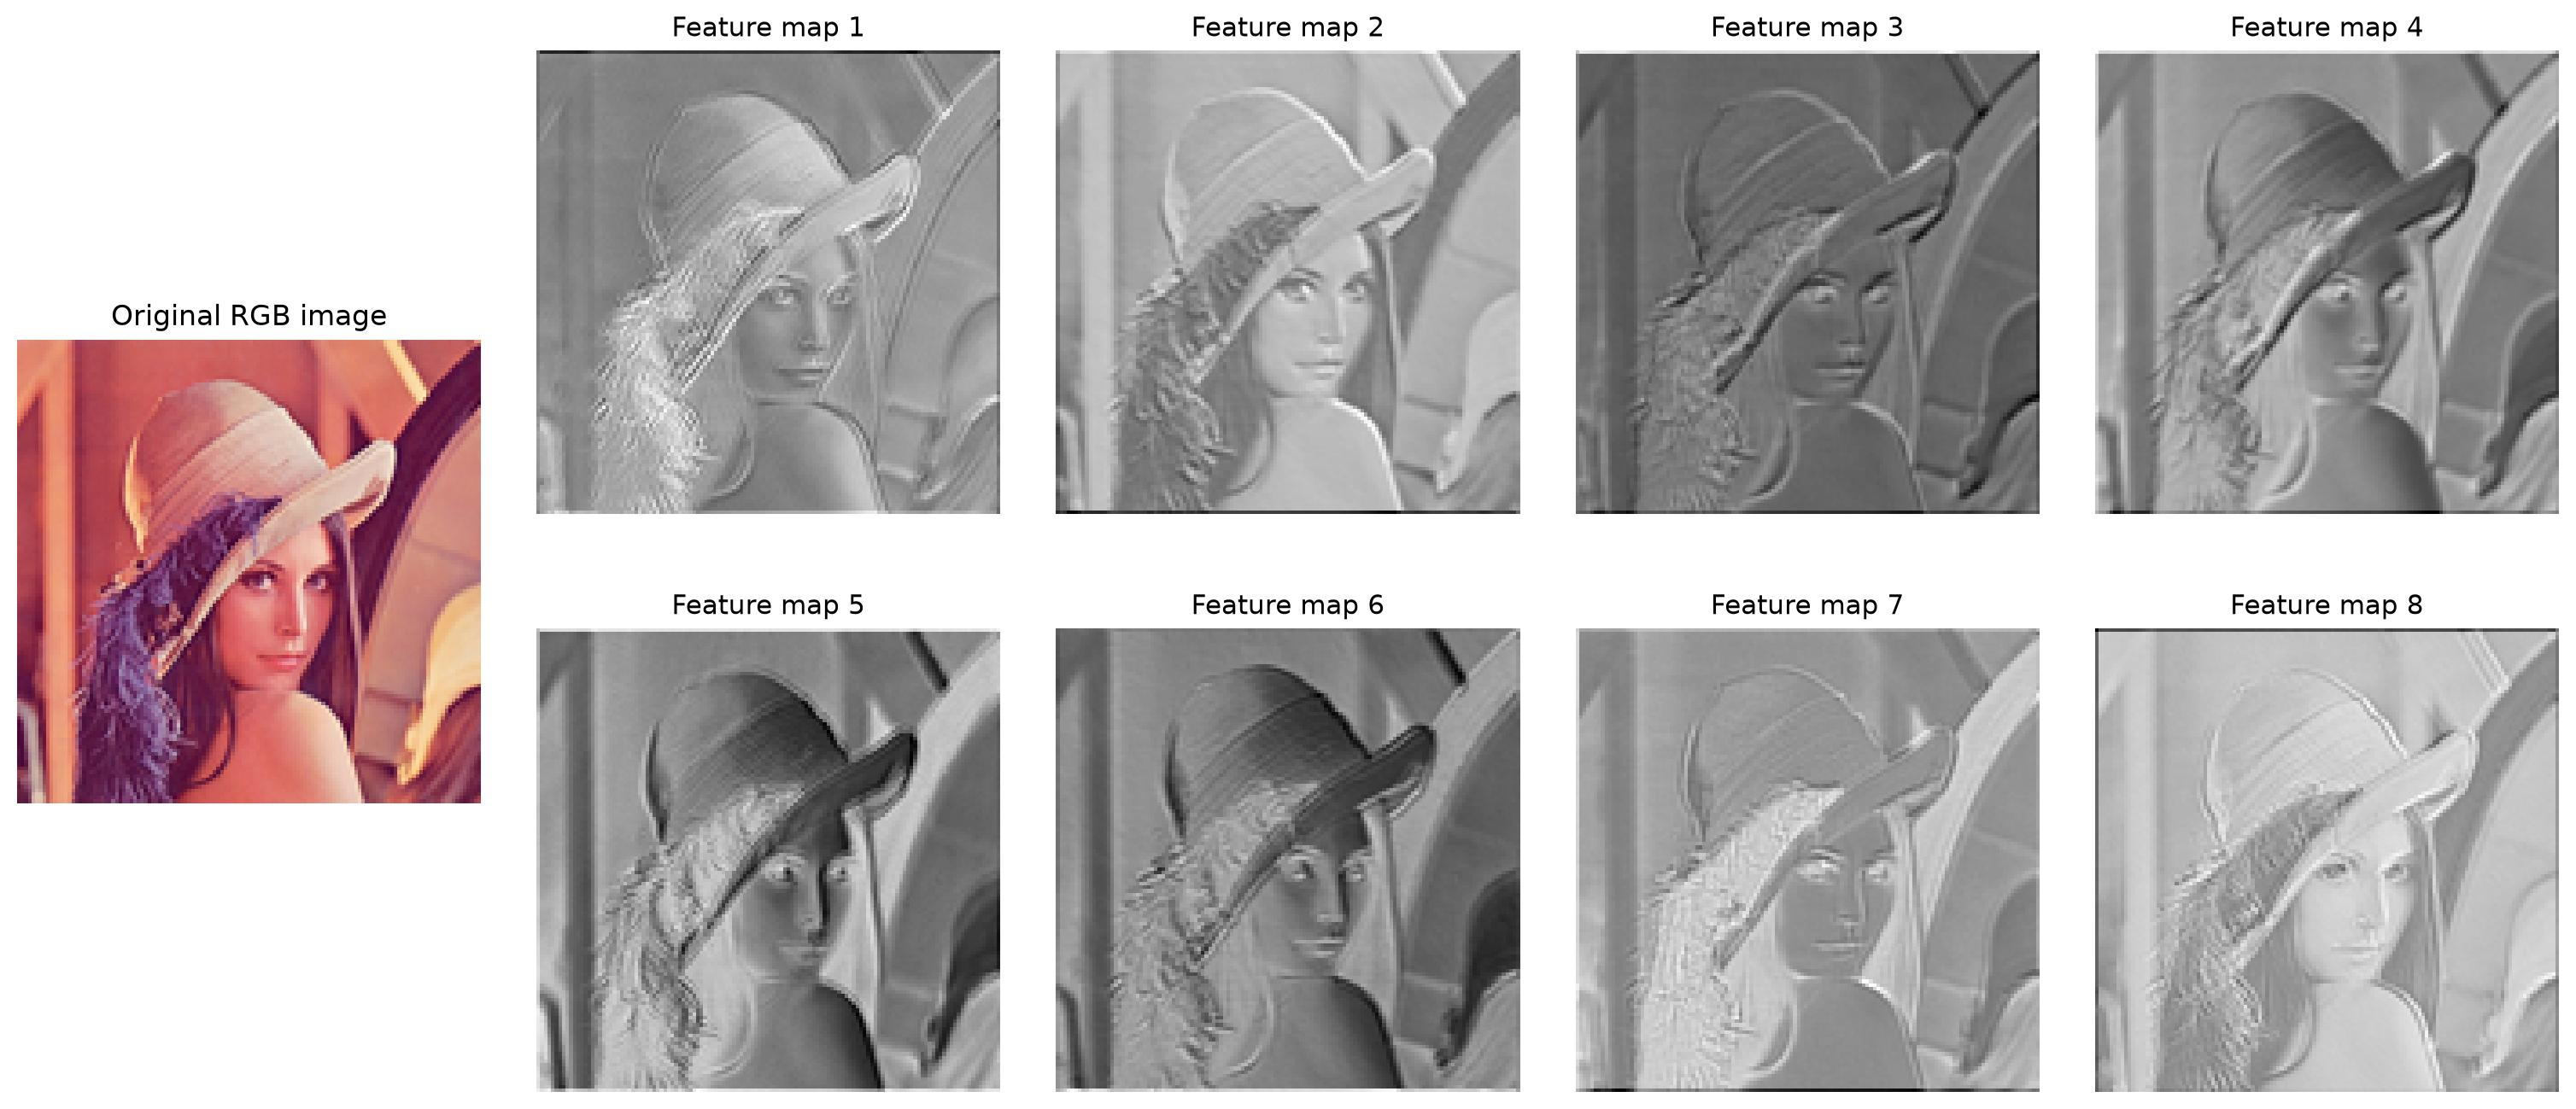
\includegraphics[width=\textwidth]{img/cnn/lena_conv1.jpg}
        \caption{Output of the first convolutional layer. Each of the 8 learned filters produces one feature map containing both positive and negative responses to local image patterns.}
        \label{fig:lena-conv1}
    \end{figure}

    \begin{figure}[!htp]
        \centering
        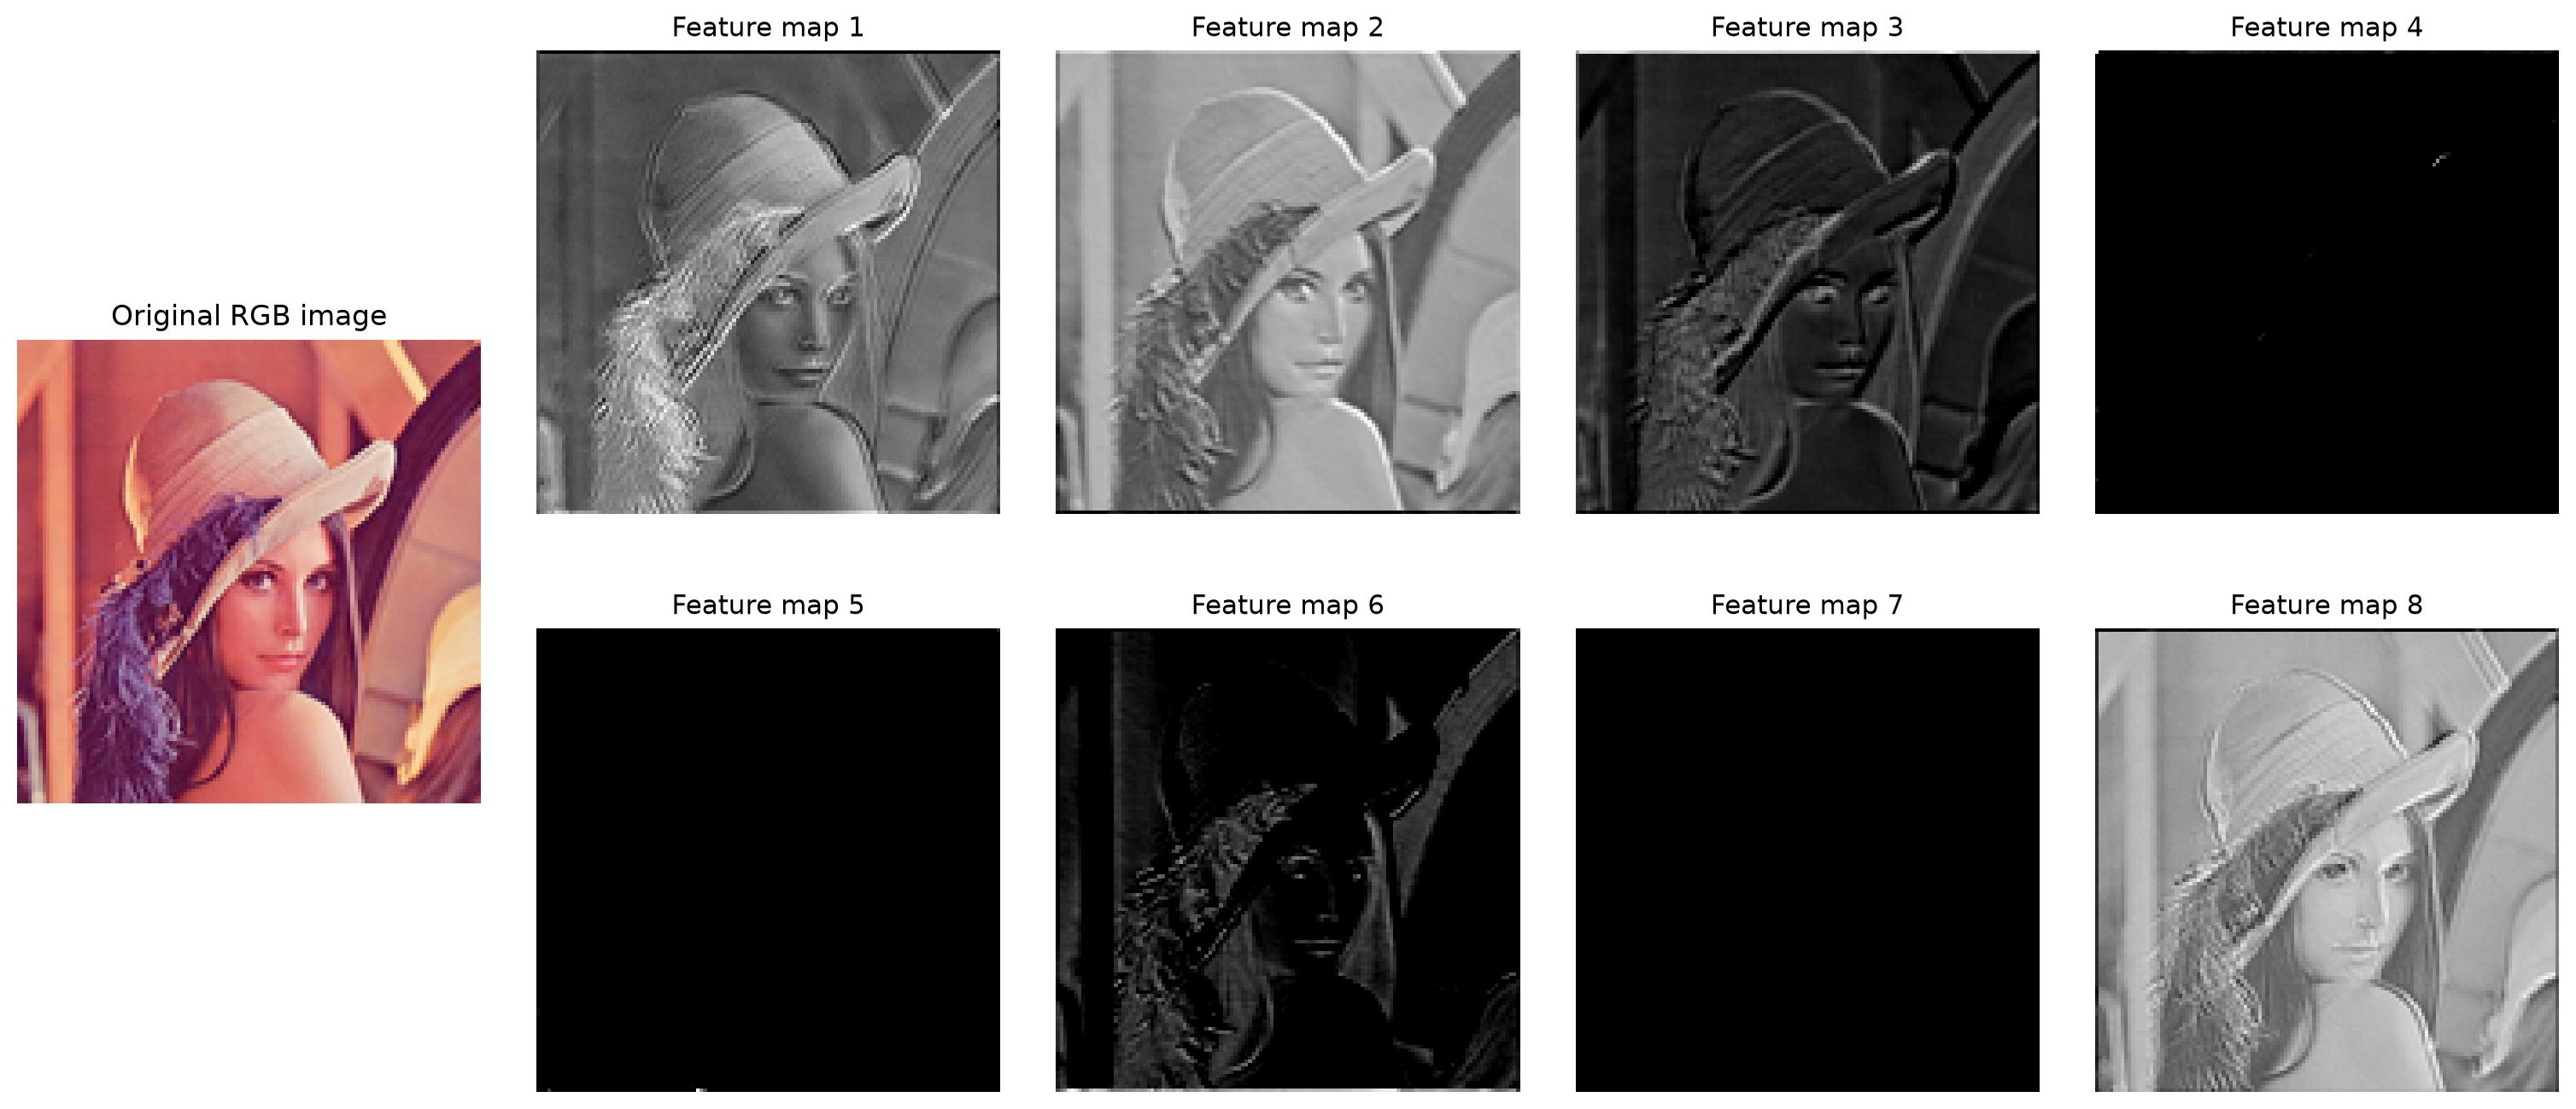
\includegraphics[width=\textwidth]{img/cnn/lena_conv1_relu.jpg}
        \caption{Output of the first convolutional layer after applying the ReLU activation function. Negative responses are set to zero, producing sparser feature maps that are passed to the subsequent layers of the CNN. The reason we apply ReLU will be explained in the following sections.}
        \label{fig:lena-conv1-relu}
    \end{figure}
    
    
    \item The second layer is a \textbf{max-pooling layer}. We do not talk about the details of pooling yet, but we can observe that the \hl{output volume has the same number of channels as the input ($8$), but the height and width are halved} ($64\times64$). Thus, pooling reduces the spatial resolution (height and width). The output of this layer is represented as $8@64\times64$.
    
    
    \item The third layer is another \textbf{convolutional layer}. It applies 24 learned filters to the input volume. The number of filters has no theoretical reason to be $24$; it is simply an example. The output volume has the same height and width as the input ($64\times64$) because we use padding. Thus, the output of this layer is represented as $24@64\times64$.
    
    
    \item The fourth layer is another \textbf{max-pooling layer}. The output volume has the same number of channels as the input ($24$), but the height and width are halved again ($16\times16$). Thus, the output of this layer is represented as $24@16\times16$.
    
    
    \item The fifth layer is a \textbf{flattening layer}. It takes the output of the previous layer, which is a volume of size $24@16\times16$, and flattens it into a one-dimensional feature vector of size $1\times6144$:
    \begin{equation*}
        24 \times 16 \times 16 = 6144
    \end{equation*}
    This is the point where the \hl{CNN transitions from spatial processing to ordinary vector processing.} 
    
    
    \item The sixth layer is a \textbf{dense layer}. It takes the feature vector of size $1\times6144$ and produces a new feature vector of size $1\times256$. This layer is \textbf{fully connected}, meaning that each of the 256 output features is computed as a weighted sum of all 6144 input features, followed by a non-linear activation function. We will discuss dense layers in detail later.
\end{itemize}
Note that these numbers are just an example, but they are \textbf{hyperparameters} that can be tuned. The \hl{network designer can choose the number of filters, the size of the filters, the number of pooling layers, and the size of the dense layers.} The \textbf{goal} is to \textbf{find a good architecture} that balances model capacity and computational efficiency.

\highspace
\textcolor{Green3}{\faIcon{question-circle} \textbf{Why does depth increase while width decreases?}} Notice the pattern:
\begin{equation*}
    3@128\times128 \to 8@128\times128 \to 8@64\times64 \to 24@64\times64 \to 24@16\times16
\end{equation*}
As we go deeper into the network, the number of channels (depth) increases, while the spatial dimensions (height and width) decrease. Two trends are at play here:
\begin{itemize}\phantomsection\label{sec:depth-increases-while-width-decreases}
    \item[\textcolor{Green3}{\faIcon{arrow-down}}] \textbf{Spatial dimensions decrease}: The image becomes smaller in height and width due to \hl{pooling layers, which reduce the spatial resolution} (i.e., how many pixels are used to represent the image). So the network is \hl{compressing \textbf{where} the information is located in the image.}
    

    \item[\textcolor{Green3}{\faIcon{arrow-up}}] \textbf{Channel depth increases}: The number of channels increases because the \hl{network learns more and more different kind of features.} Each channel becomes a learned feature detector that responds to specific patterns in the input image. In general, \hl{each channel answers a different learned question about the input image.}
\end{itemize}
A typical architecture therefore follows the pattern:
\begin{equation*}
    H_1 \times W_1 \times C_1 \to H_2 \times W_2 \times C_2 \to H_3 \times W_3 \times C_3 \to \ldots
\end{equation*}
Where usually:
\begin{equation*}
    H_{l+1} \leq H_l, \quad W_{l+1} \leq W_l
\end{equation*}
The height and width decrease, while the number of channels increases:
\begin{equation*}
    C_{l+1} \geq C_l
\end{equation*}
In other words, \hl{smaller spatial maps, but more feature channels.}

\highspace
\begin{takeawaysbox}
    \begin{itemize}
        \item A CNN receives the complete image directly.
        \item An input image is represented as a volume:
        \begin{equation*}
            H \times W \times C
        \end{equation*}
        \item $H$ and $W$ are spatial dimensions; $C$ is the number of channels (depth).
        \item A convolutional layer applies many learned filters to the input volume.
        \item Each filter produces one output channel (feature map).
        \begin{equation*}
            \text{output depth} = \text{number of filters}
        \end{equation*}
        \item Intermediate channels represent learned features, not necessarily RGB information.
        \item A common CNN pattern is: spatial dimensions decrease while channel depth increases.
        \item Pooling typically reduces height and width without changing channel count.
        \item Convolution can change channel depth by changing the number of filters.
        \item The final volume is converted into a vector, usually through flattening:
        \begin{equation*}
            H \times W \times C \to 1 \times (H \cdot W \cdot C)
        \end{equation*}
        \item The resulting vector is fed to a traditional neural network classifier (dense layers).
        \item The complete image transformation is: (1) image to (2) sequence of feature volumes to (3) feature vector to (4) classification.
    \end{itemize}
\end{takeawaysbox}